% Created by tikzDevice version 0.12.3.1 on 2021-06-16 15:27:58
% !TEX encoding = UTF-8 Unicode
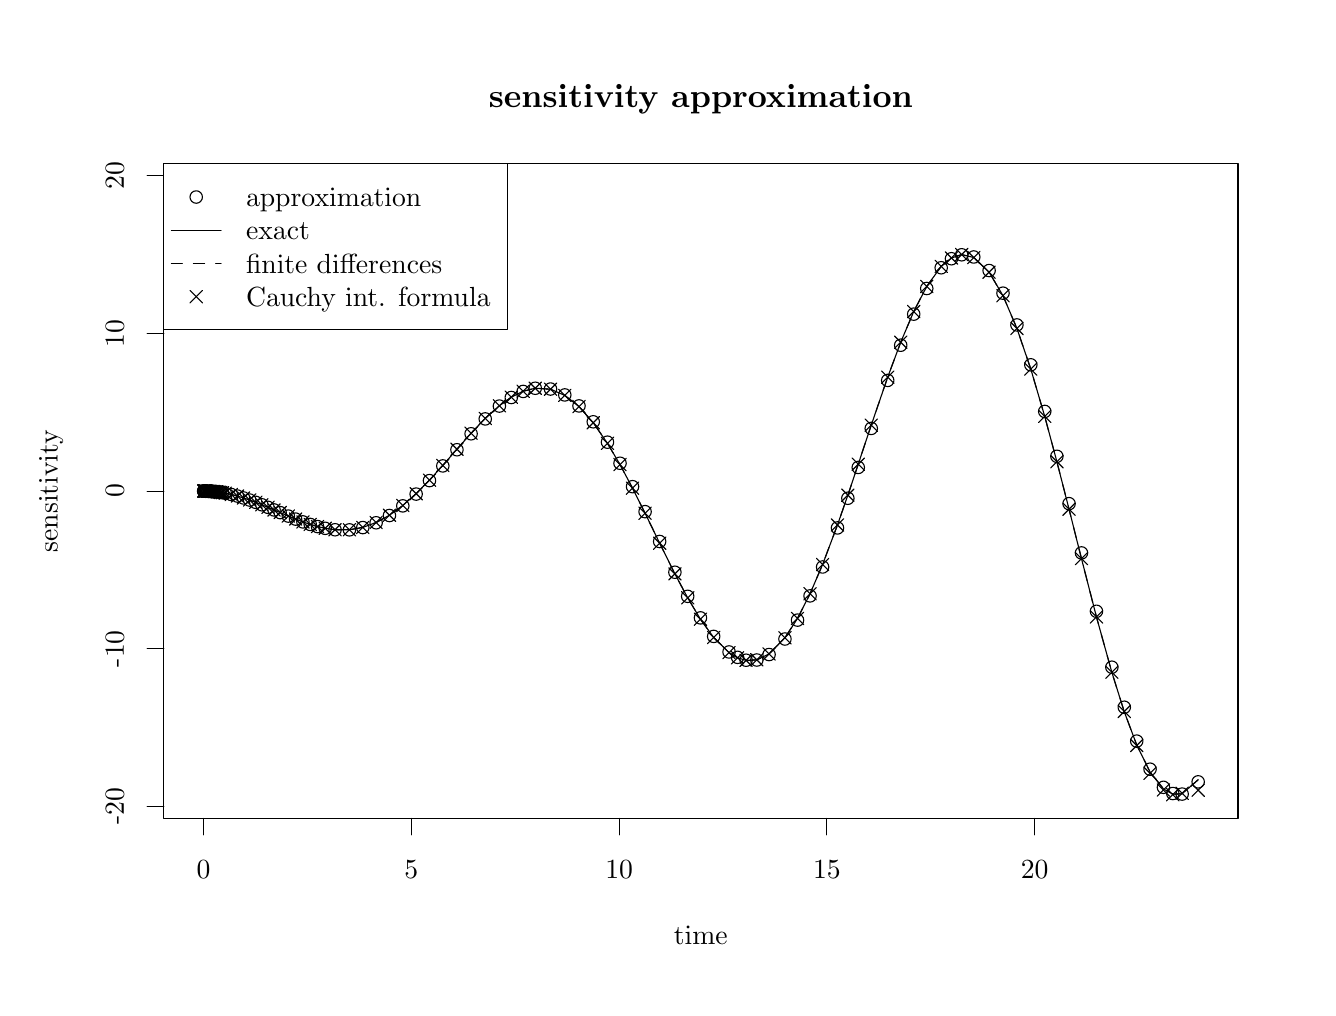
\begin{tikzpicture}[x=1pt,y=1pt]
\definecolor{fillColor}{RGB}{255,255,255}
\path[use as bounding box,fill=fillColor,fill opacity=0.00] (0,0) rectangle (462.53,346.90);
\begin{scope}
\path[clip] ( 49.20, 61.20) rectangle (437.33,297.70);
\definecolor{drawColor}{RGB}{0,0,0}

\path[draw=drawColor,line width= 0.4pt,line join=round,line cap=round] ( 63.58,179.45) circle (  2.25);

\path[draw=drawColor,line width= 0.4pt,line join=round,line cap=round] ( 63.66,179.45) circle (  2.25);

\path[draw=drawColor,line width= 0.4pt,line join=round,line cap=round] ( 63.76,179.45) circle (  2.25);

\path[draw=drawColor,line width= 0.4pt,line join=round,line cap=round] ( 63.86,179.45) circle (  2.25);

\path[draw=drawColor,line width= 0.4pt,line join=round,line cap=round] ( 63.97,179.45) circle (  2.25);

\path[draw=drawColor,line width= 0.4pt,line join=round,line cap=round] ( 64.07,179.44) circle (  2.25);

\path[draw=drawColor,line width= 0.4pt,line join=round,line cap=round] ( 64.18,179.44) circle (  2.25);

\path[draw=drawColor,line width= 0.4pt,line join=round,line cap=round] ( 64.28,179.44) circle (  2.25);

\path[draw=drawColor,line width= 0.4pt,line join=round,line cap=round] ( 64.43,179.44) circle (  2.25);

\path[draw=drawColor,line width= 0.4pt,line join=round,line cap=round] ( 64.66,179.43) circle (  2.25);

\path[draw=drawColor,line width= 0.4pt,line join=round,line cap=round] ( 65.06,179.42) circle (  2.25);

\path[draw=drawColor,line width= 0.4pt,line join=round,line cap=round] ( 65.57,179.40) circle (  2.25);

\path[draw=drawColor,line width= 0.4pt,line join=round,line cap=round] ( 66.09,179.37) circle (  2.25);

\path[draw=drawColor,line width= 0.4pt,line join=round,line cap=round] ( 66.61,179.33) circle (  2.25);

\path[draw=drawColor,line width= 0.4pt,line join=round,line cap=round] ( 67.13,179.29) circle (  2.25);

\path[draw=drawColor,line width= 0.4pt,line join=round,line cap=round] ( 67.65,179.24) circle (  2.25);

\path[draw=drawColor,line width= 0.4pt,line join=round,line cap=round] ( 68.17,179.18) circle (  2.25);

\path[draw=drawColor,line width= 0.4pt,line join=round,line cap=round] ( 68.69,179.12) circle (  2.25);

\path[draw=drawColor,line width= 0.4pt,line join=round,line cap=round] ( 69.21,179.05) circle (  2.25);

\path[draw=drawColor,line width= 0.4pt,line join=round,line cap=round] ( 69.73,178.97) circle (  2.25);

\path[draw=drawColor,line width= 0.4pt,line join=round,line cap=round] ( 70.38,178.87) circle (  2.25);

\path[draw=drawColor,line width= 0.4pt,line join=round,line cap=round] ( 71.38,178.69) circle (  2.25);

\path[draw=drawColor,line width= 0.4pt,line join=round,line cap=round] ( 73.59,178.21) circle (  2.25);

\path[draw=drawColor,line width= 0.4pt,line join=round,line cap=round] ( 75.80,177.64) circle (  2.25);

\path[draw=drawColor,line width= 0.4pt,line join=round,line cap=round] ( 78.00,176.96) circle (  2.25);

\path[draw=drawColor,line width= 0.4pt,line join=round,line cap=round] ( 80.21,176.21) circle (  2.25);

\path[draw=drawColor,line width= 0.4pt,line join=round,line cap=round] ( 82.41,175.38) circle (  2.25);

\path[draw=drawColor,line width= 0.4pt,line join=round,line cap=round] ( 84.62,174.50) circle (  2.25);

\path[draw=drawColor,line width= 0.4pt,line join=round,line cap=round] ( 86.83,173.58) circle (  2.25);

\path[draw=drawColor,line width= 0.4pt,line join=round,line cap=round] ( 89.03,172.63) circle (  2.25);

\path[draw=drawColor,line width= 0.4pt,line join=round,line cap=round] ( 91.24,171.67) circle (  2.25);

\path[draw=drawColor,line width= 0.4pt,line join=round,line cap=round] ( 94.18,170.41) circle (  2.25);

\path[draw=drawColor,line width= 0.4pt,line join=round,line cap=round] ( 96.82,169.32) circle (  2.25);

\path[draw=drawColor,line width= 0.4pt,line join=round,line cap=round] ( 99.46,168.31) circle (  2.25);

\path[draw=drawColor,line width= 0.4pt,line join=round,line cap=round] (102.10,167.40) circle (  2.25);

\path[draw=drawColor,line width= 0.4pt,line join=round,line cap=round] (104.74,166.62) circle (  2.25);

\path[draw=drawColor,line width= 0.4pt,line join=round,line cap=round] (107.51,165.99) circle (  2.25);

\path[draw=drawColor,line width= 0.4pt,line join=round,line cap=round] (111.06,165.47) circle (  2.25);

\path[draw=drawColor,line width= 0.4pt,line join=round,line cap=round] (116.27,165.43) circle (  2.25);

\path[draw=drawColor,line width= 0.4pt,line join=round,line cap=round] (121.09,166.26) circle (  2.25);

\path[draw=drawColor,line width= 0.4pt,line join=round,line cap=round] (125.91,167.99) circle (  2.25);

\path[draw=drawColor,line width= 0.4pt,line join=round,line cap=round] (130.73,170.62) circle (  2.25);

\path[draw=drawColor,line width= 0.4pt,line join=round,line cap=round] (135.55,174.10) circle (  2.25);

\path[draw=drawColor,line width= 0.4pt,line join=round,line cap=round] (140.37,178.36) circle (  2.25);

\path[draw=drawColor,line width= 0.4pt,line join=round,line cap=round] (145.19,183.23) circle (  2.25);

\path[draw=drawColor,line width= 0.4pt,line join=round,line cap=round] (150.01,188.54) circle (  2.25);

\path[draw=drawColor,line width= 0.4pt,line join=round,line cap=round] (155.12,194.38) circle (  2.25);

\path[draw=drawColor,line width= 0.4pt,line join=round,line cap=round] (160.23,200.15) circle (  2.25);

\path[draw=drawColor,line width= 0.4pt,line join=round,line cap=round] (165.34,205.52) circle (  2.25);

\path[draw=drawColor,line width= 0.4pt,line join=round,line cap=round] (170.45,210.16) circle (  2.25);

\path[draw=drawColor,line width= 0.4pt,line join=round,line cap=round] (174.75,213.26) circle (  2.25);

\path[draw=drawColor,line width= 0.4pt,line join=round,line cap=round] (179.05,215.45) circle (  2.25);

\path[draw=drawColor,line width= 0.4pt,line join=round,line cap=round] (183.41,216.60) circle (  2.25);

\path[draw=drawColor,line width= 0.4pt,line join=round,line cap=round] (188.93,216.32) circle (  2.25);

\path[draw=drawColor,line width= 0.4pt,line join=round,line cap=round] (194.08,214.19) circle (  2.25);

\path[draw=drawColor,line width= 0.4pt,line join=round,line cap=round] (199.22,210.22) circle (  2.25);

\path[draw=drawColor,line width= 0.4pt,line join=round,line cap=round] (204.37,204.48) circle (  2.25);

\path[draw=drawColor,line width= 0.4pt,line join=round,line cap=round] (209.51,197.12) circle (  2.25);

\path[draw=drawColor,line width= 0.4pt,line join=round,line cap=round] (214.04,189.50) circle (  2.25);

\path[draw=drawColor,line width= 0.4pt,line join=round,line cap=round] (218.57,181.04) circle (  2.25);

\path[draw=drawColor,line width= 0.4pt,line join=round,line cap=round] (223.10,172.01) circle (  2.25);

\path[draw=drawColor,line width= 0.4pt,line join=round,line cap=round] (228.36,161.23) circle (  2.25);

\path[draw=drawColor,line width= 0.4pt,line join=round,line cap=round] (233.87,150.12) circle (  2.25);

\path[draw=drawColor,line width= 0.4pt,line join=round,line cap=round] (238.49,141.41) circle (  2.25);

\path[draw=drawColor,line width= 0.4pt,line join=round,line cap=round] (243.11,133.63) circle (  2.25);

\path[draw=drawColor,line width= 0.4pt,line join=round,line cap=round] (247.88,126.94) circle (  2.25);

\path[draw=drawColor,line width= 0.4pt,line join=round,line cap=round] (253.44,121.31) circle (  2.25);

\path[draw=drawColor,line width= 0.4pt,line join=round,line cap=round] (256.52,119.37) circle (  2.25);

\path[draw=drawColor,line width= 0.4pt,line join=round,line cap=round] (259.60,118.33) circle (  2.25);

\path[draw=drawColor,line width= 0.4pt,line join=round,line cap=round] (263.48,118.40) circle (  2.25);

\path[draw=drawColor,line width= 0.4pt,line join=round,line cap=round] (267.90,120.38) circle (  2.25);

\path[draw=drawColor,line width= 0.4pt,line join=round,line cap=round] (273.64,125.99) circle (  2.25);

\path[draw=drawColor,line width= 0.4pt,line join=round,line cap=round] (278.18,132.82) circle (  2.25);

\path[draw=drawColor,line width= 0.4pt,line join=round,line cap=round] (282.71,141.57) circle (  2.25);

\path[draw=drawColor,line width= 0.4pt,line join=round,line cap=round] (287.25,152.02) circle (  2.25);

\path[draw=drawColor,line width= 0.4pt,line join=round,line cap=round] (292.62,166.13) circle (  2.25);

\path[draw=drawColor,line width= 0.4pt,line join=round,line cap=round] (296.37,176.85) circle (  2.25);

\path[draw=drawColor,line width= 0.4pt,line join=round,line cap=round] (300.13,187.99) circle (  2.25);

\path[draw=drawColor,line width= 0.4pt,line join=round,line cap=round] (304.82,202.09) circle (  2.25);

\path[draw=drawColor,line width= 0.4pt,line join=round,line cap=round] (310.77,219.44) circle (  2.25);

\path[draw=drawColor,line width= 0.4pt,line join=round,line cap=round] (315.47,232.15) circle (  2.25);

\path[draw=drawColor,line width= 0.4pt,line join=round,line cap=round] (320.17,243.38) circle (  2.25);

\path[draw=drawColor,line width= 0.4pt,line join=round,line cap=round] (324.88,252.65) circle (  2.25);

\path[draw=drawColor,line width= 0.4pt,line join=round,line cap=round] (330.10,260.14) circle (  2.25);

\path[draw=drawColor,line width= 0.4pt,line join=round,line cap=round] (333.80,263.40) circle (  2.25);

\path[draw=drawColor,line width= 0.4pt,line join=round,line cap=round] (337.50,264.83) circle (  2.25);

\path[draw=drawColor,line width= 0.4pt,line join=round,line cap=round] (341.87,264.04) circle (  2.25);

\path[draw=drawColor,line width= 0.4pt,line join=round,line cap=round] (347.41,259.14) circle (  2.25);

\path[draw=drawColor,line width= 0.4pt,line join=round,line cap=round] (352.43,250.96) circle (  2.25);

\path[draw=drawColor,line width= 0.4pt,line join=round,line cap=round] (357.46,239.48) circle (  2.25);

\path[draw=drawColor,line width= 0.4pt,line join=round,line cap=round] (362.48,225.07) circle (  2.25);

\path[draw=drawColor,line width= 0.4pt,line join=round,line cap=round] (367.51,208.23) circle (  2.25);

\path[draw=drawColor,line width= 0.4pt,line join=round,line cap=round] (371.90,192.01) circle (  2.25);

\path[draw=drawColor,line width= 0.4pt,line join=round,line cap=round] (376.30,174.90) circle (  2.25);

\path[draw=drawColor,line width= 0.4pt,line join=round,line cap=round] (380.79,157.10) circle (  2.25);

\path[draw=drawColor,line width= 0.4pt,line join=round,line cap=round] (386.20,136.01) circle (  2.25);

\path[draw=drawColor,line width= 0.4pt,line join=round,line cap=round] (391.77,115.80) circle (  2.25);

\path[draw=drawColor,line width= 0.4pt,line join=round,line cap=round] (396.26,101.34) circle (  2.25);

\path[draw=drawColor,line width= 0.4pt,line join=round,line cap=round] (400.75, 89.10) circle (  2.25);

\path[draw=drawColor,line width= 0.4pt,line join=round,line cap=round] (405.57, 78.95) circle (  2.25);

\path[draw=drawColor,line width= 0.4pt,line join=round,line cap=round] (410.40, 72.40) circle (  2.25);

\path[draw=drawColor,line width= 0.4pt,line join=round,line cap=round] (413.79, 70.16) circle (  2.25);

\path[draw=drawColor,line width= 0.4pt,line join=round,line cap=round] (417.17, 69.96) circle (  2.25);

\path[draw=drawColor,line width= 0.4pt,line join=round,line cap=round] (422.95, 74.38) circle (  2.25);
\end{scope}
\begin{scope}
\path[clip] (  0.00,  0.00) rectangle (462.53,346.90);
\definecolor{drawColor}{RGB}{0,0,0}

\path[draw=drawColor,line width= 0.4pt,line join=round,line cap=round] ( 63.58, 61.20) -- (363.85, 61.20);

\path[draw=drawColor,line width= 0.4pt,line join=round,line cap=round] ( 63.58, 61.20) -- ( 63.58, 55.20);

\path[draw=drawColor,line width= 0.4pt,line join=round,line cap=round] (138.64, 61.20) -- (138.64, 55.20);

\path[draw=drawColor,line width= 0.4pt,line join=round,line cap=round] (213.71, 61.20) -- (213.71, 55.20);

\path[draw=drawColor,line width= 0.4pt,line join=round,line cap=round] (288.78, 61.20) -- (288.78, 55.20);

\path[draw=drawColor,line width= 0.4pt,line join=round,line cap=round] (363.85, 61.20) -- (363.85, 55.20);

\node[text=drawColor,anchor=base,inner sep=0pt, outer sep=0pt, scale=  1.00] at ( 63.58, 39.60) {0};

\node[text=drawColor,anchor=base,inner sep=0pt, outer sep=0pt, scale=  1.00] at (138.64, 39.60) {5};

\node[text=drawColor,anchor=base,inner sep=0pt, outer sep=0pt, scale=  1.00] at (213.71, 39.60) {10};

\node[text=drawColor,anchor=base,inner sep=0pt, outer sep=0pt, scale=  1.00] at (288.78, 39.60) {15};

\node[text=drawColor,anchor=base,inner sep=0pt, outer sep=0pt, scale=  1.00] at (363.85, 39.60) {20};

\path[draw=drawColor,line width= 0.4pt,line join=round,line cap=round] ( 49.20, 65.53) -- ( 49.20,293.36);

\path[draw=drawColor,line width= 0.4pt,line join=round,line cap=round] ( 49.20, 65.53) -- ( 43.20, 65.53);

\path[draw=drawColor,line width= 0.4pt,line join=round,line cap=round] ( 49.20,122.49) -- ( 43.20,122.49);

\path[draw=drawColor,line width= 0.4pt,line join=round,line cap=round] ( 49.20,179.45) -- ( 43.20,179.45);

\path[draw=drawColor,line width= 0.4pt,line join=round,line cap=round] ( 49.20,236.41) -- ( 43.20,236.41);

\path[draw=drawColor,line width= 0.4pt,line join=round,line cap=round] ( 49.20,293.36) -- ( 43.20,293.36);

\node[text=drawColor,rotate= 90.00,anchor=base,inner sep=0pt, outer sep=0pt, scale=  1.00] at ( 34.80, 65.53) {-20};

\node[text=drawColor,rotate= 90.00,anchor=base,inner sep=0pt, outer sep=0pt, scale=  1.00] at ( 34.80,122.49) {-10};

\node[text=drawColor,rotate= 90.00,anchor=base,inner sep=0pt, outer sep=0pt, scale=  1.00] at ( 34.80,179.45) {0};

\node[text=drawColor,rotate= 90.00,anchor=base,inner sep=0pt, outer sep=0pt, scale=  1.00] at ( 34.80,236.41) {10};

\node[text=drawColor,rotate= 90.00,anchor=base,inner sep=0pt, outer sep=0pt, scale=  1.00] at ( 34.80,293.36) {20};

\path[draw=drawColor,line width= 0.4pt,line join=round,line cap=round] ( 49.20, 61.20) --
	(437.33, 61.20) --
	(437.33,297.70) --
	( 49.20,297.70) --
	( 49.20, 61.20);
\end{scope}
\begin{scope}
\path[clip] (  0.00,  0.00) rectangle (462.53,346.90);
\definecolor{drawColor}{RGB}{0,0,0}

\node[text=drawColor,anchor=base,inner sep=0pt, outer sep=0pt, scale=  1.20] at (243.26,318.16) {\bfseries sensitivity approximation};

\node[text=drawColor,anchor=base,inner sep=0pt, outer sep=0pt, scale=  1.00] at (243.26, 15.60) {time};

\node[text=drawColor,rotate= 90.00,anchor=base,inner sep=0pt, outer sep=0pt, scale=  1.00] at ( 10.80,179.45) {sensitivity};
\end{scope}
\begin{scope}
\path[clip] ( 49.20, 61.20) rectangle (437.33,297.70);
\definecolor{drawColor}{RGB}{0,0,0}

\path[draw=drawColor,line width= 0.4pt,line join=round,line cap=round] ( 63.58,179.45) --
	( 63.66,179.45) --
	( 63.76,179.45) --
	( 63.86,179.45) --
	( 63.97,179.45) --
	( 64.07,179.44) --
	( 64.18,179.44) --
	( 64.28,179.44) --
	( 64.43,179.44) --
	( 64.66,179.43) --
	( 65.06,179.42) --
	( 65.57,179.40) --
	( 66.09,179.37) --
	( 66.61,179.33) --
	( 67.13,179.29) --
	( 67.65,179.24) --
	( 68.17,179.18) --
	( 68.69,179.12) --
	( 69.21,179.05) --
	( 69.73,178.97) --
	( 70.38,178.87) --
	( 71.38,178.69) --
	( 73.59,178.22) --
	( 75.80,177.64) --
	( 78.00,176.96) --
	( 80.21,176.21) --
	( 82.41,175.38) --
	( 84.62,174.50) --
	( 86.83,173.58) --
	( 89.03,172.63) --
	( 91.24,171.67) --
	( 94.18,170.41) --
	( 96.82,169.32) --
	( 99.46,168.31) --
	(102.10,167.40) --
	(104.74,166.63) --
	(107.51,165.99) --
	(111.06,165.49) --
	(116.27,165.47) --
	(121.09,166.32) --
	(125.91,168.07) --
	(130.73,170.72) --
	(135.55,174.23) --
	(140.37,178.51) --
	(145.19,183.40) --
	(150.01,188.73) --
	(155.12,194.58) --
	(160.23,200.34) --
	(165.34,205.70) --
	(170.45,210.30) --
	(174.75,213.37) --
	(179.05,215.52) --
	(183.41,216.61) --
	(188.93,216.25) --
	(194.08,214.03) --
	(199.22,209.97) --
	(204.37,204.14) --
	(209.51,196.69) --
	(214.04,189.01) --
	(218.57,180.50) --
	(223.10,171.44) --
	(228.36,160.63) --
	(233.87,149.53) --
	(238.49,140.86) --
	(243.11,133.14) --
	(247.88,126.55) --
	(253.44,121.07) --
	(256.52,119.21) --
	(259.60,118.27) --
	(263.48,118.46) --
	(267.90,120.61) --
	(273.64,126.45) --
	(278.18,133.44) --
	(282.71,142.35) --
	(287.25,152.94) --
	(292.62,167.20) --
	(296.37,177.98) --
	(300.13,189.15) --
	(304.82,203.27) --
	(310.77,220.61) --
	(315.47,233.23) --
	(320.17,244.32) --
	(324.88,253.41) --
	(330.10,260.64) --
	(333.80,263.69) --
	(337.50,264.90) --
	(341.87,263.84) --
	(347.41,258.55) --
	(352.43,250.04) --
	(357.46,238.23) --
	(362.48,223.52) --
	(367.51,206.44) --
	(371.90,190.07) --
	(376.30,172.88) --
	(380.79,155.04) --
	(386.20,133.98) --
	(391.77,113.92) --
	(396.26, 99.68) --
	(400.75, 87.72) --
	(405.57, 77.95) --
	(410.40, 71.84) --
	(413.79, 69.93) --
	(417.17, 70.07) --
	(422.95, 75.13);

\path[draw=drawColor,line width= 0.4pt,dash pattern=on 4pt off 4pt ,line join=round,line cap=round] ( 63.58,179.45) --
	( 63.66,179.45) --
	( 63.76,179.45) --
	( 63.86,179.45) --
	( 63.97,179.45) --
	( 64.07,179.44) --
	( 64.18,179.44) --
	( 64.28,179.44) --
	( 64.43,179.44) --
	( 64.66,179.43) --
	( 65.06,179.42) --
	( 65.57,179.40) --
	( 66.09,179.37) --
	( 66.61,179.33) --
	( 67.13,179.29) --
	( 67.65,179.24) --
	( 68.17,179.18) --
	( 68.69,179.12) --
	( 69.21,179.05) --
	( 69.73,178.97) --
	( 70.38,178.87) --
	( 71.38,178.69) --
	( 73.59,178.22) --
	( 75.80,177.64) --
	( 78.00,176.96) --
	( 80.21,176.21) --
	( 82.41,175.38) --
	( 84.62,174.50) --
	( 86.83,173.58) --
	( 89.03,172.63) --
	( 91.24,171.67) --
	( 94.18,170.41) --
	( 96.82,169.32) --
	( 99.46,168.31) --
	(102.10,167.40) --
	(104.74,166.63) --
	(107.51,165.99) --
	(111.06,165.49) --
	(116.27,165.47) --
	(121.09,166.32) --
	(125.91,168.07) --
	(130.73,170.72) --
	(135.55,174.23) --
	(140.37,178.51) --
	(145.19,183.40) --
	(150.01,188.73) --
	(155.12,194.58) --
	(160.23,200.34) --
	(165.34,205.70) --
	(170.45,210.30) --
	(174.75,213.37) --
	(179.05,215.52) --
	(183.41,216.61) --
	(188.93,216.25) --
	(194.08,214.03) --
	(199.22,209.97) --
	(204.37,204.14) --
	(209.51,196.69) --
	(214.04,189.01) --
	(218.57,180.50) --
	(223.10,171.44) --
	(228.36,160.63) --
	(233.87,149.53) --
	(238.49,140.86) --
	(243.11,133.14) --
	(247.88,126.55) --
	(253.44,121.07) --
	(256.52,119.21) --
	(259.60,118.27) --
	(263.48,118.46) --
	(267.90,120.61) --
	(273.64,126.45) --
	(278.18,133.44) --
	(282.71,142.35) --
	(287.25,152.94) --
	(292.62,167.20) --
	(296.37,177.98) --
	(300.13,189.15) --
	(304.82,203.27) --
	(310.77,220.61) --
	(315.47,233.23) --
	(320.17,244.32) --
	(324.88,253.41) --
	(330.10,260.64) --
	(333.80,263.69) --
	(337.50,264.90) --
	(341.87,263.84) --
	(347.41,258.55) --
	(352.43,250.04) --
	(357.46,238.23) --
	(362.48,223.52) --
	(367.51,206.44) --
	(371.90,190.07) --
	(376.30,172.88) --
	(380.79,155.04) --
	(386.20,133.98) --
	(391.77,113.92) --
	(396.26, 99.68) --
	(400.75, 87.72) --
	(405.57, 77.95) --
	(410.40, 71.84) --
	(413.79, 69.93) --
	(417.17, 70.07) --
	(422.95, 75.13);

\path[draw=drawColor,line width= 0.4pt,line join=round,line cap=round] ( 61.33,177.20) -- ( 65.83,181.70);

\path[draw=drawColor,line width= 0.4pt,line join=round,line cap=round] ( 61.33,181.70) -- ( 65.83,177.20);

\path[draw=drawColor,line width= 0.4pt,line join=round,line cap=round] ( 61.41,177.20) -- ( 65.91,181.70);

\path[draw=drawColor,line width= 0.4pt,line join=round,line cap=round] ( 61.41,181.70) -- ( 65.91,177.20);

\path[draw=drawColor,line width= 0.4pt,line join=round,line cap=round] ( 61.51,177.20) -- ( 66.01,181.70);

\path[draw=drawColor,line width= 0.4pt,line join=round,line cap=round] ( 61.51,181.70) -- ( 66.01,177.20);

\path[draw=drawColor,line width= 0.4pt,line join=round,line cap=round] ( 61.61,177.20) -- ( 66.11,181.70);

\path[draw=drawColor,line width= 0.4pt,line join=round,line cap=round] ( 61.61,181.70) -- ( 66.11,177.20);

\path[draw=drawColor,line width= 0.4pt,line join=round,line cap=round] ( 61.72,177.20) -- ( 66.22,181.70);

\path[draw=drawColor,line width= 0.4pt,line join=round,line cap=round] ( 61.72,181.70) -- ( 66.22,177.20);

\path[draw=drawColor,line width= 0.4pt,line join=round,line cap=round] ( 61.82,177.19) -- ( 66.32,181.69);

\path[draw=drawColor,line width= 0.4pt,line join=round,line cap=round] ( 61.82,181.69) -- ( 66.32,177.19);

\path[draw=drawColor,line width= 0.4pt,line join=round,line cap=round] ( 61.93,177.19) -- ( 66.43,181.69);

\path[draw=drawColor,line width= 0.4pt,line join=round,line cap=round] ( 61.93,181.69) -- ( 66.43,177.19);

\path[draw=drawColor,line width= 0.4pt,line join=round,line cap=round] ( 62.03,177.19) -- ( 66.53,181.69);

\path[draw=drawColor,line width= 0.4pt,line join=round,line cap=round] ( 62.03,181.69) -- ( 66.53,177.19);

\path[draw=drawColor,line width= 0.4pt,line join=round,line cap=round] ( 62.18,177.19) -- ( 66.68,181.69);

\path[draw=drawColor,line width= 0.4pt,line join=round,line cap=round] ( 62.18,181.69) -- ( 66.68,177.19);

\path[draw=drawColor,line width= 0.4pt,line join=round,line cap=round] ( 62.41,177.18) -- ( 66.91,181.68);

\path[draw=drawColor,line width= 0.4pt,line join=round,line cap=round] ( 62.41,181.68) -- ( 66.91,177.18);

\path[draw=drawColor,line width= 0.4pt,line join=round,line cap=round] ( 62.81,177.17) -- ( 67.31,181.67);

\path[draw=drawColor,line width= 0.4pt,line join=round,line cap=round] ( 62.81,181.67) -- ( 67.31,177.17);

\path[draw=drawColor,line width= 0.4pt,line join=round,line cap=round] ( 63.32,177.15) -- ( 67.82,181.65);

\path[draw=drawColor,line width= 0.4pt,line join=round,line cap=round] ( 63.32,181.65) -- ( 67.82,177.15);

\path[draw=drawColor,line width= 0.4pt,line join=round,line cap=round] ( 63.84,177.12) -- ( 68.34,181.62);

\path[draw=drawColor,line width= 0.4pt,line join=round,line cap=round] ( 63.84,181.62) -- ( 68.34,177.12);

\path[draw=drawColor,line width= 0.4pt,line join=round,line cap=round] ( 64.36,177.08) -- ( 68.86,181.58);

\path[draw=drawColor,line width= 0.4pt,line join=round,line cap=round] ( 64.36,181.58) -- ( 68.86,177.08);

\path[draw=drawColor,line width= 0.4pt,line join=round,line cap=round] ( 64.88,177.04) -- ( 69.38,181.54);

\path[draw=drawColor,line width= 0.4pt,line join=round,line cap=round] ( 64.88,181.54) -- ( 69.38,177.04);

\path[draw=drawColor,line width= 0.4pt,line join=round,line cap=round] ( 65.40,176.99) -- ( 69.90,181.49);

\path[draw=drawColor,line width= 0.4pt,line join=round,line cap=round] ( 65.40,181.49) -- ( 69.90,176.99);

\path[draw=drawColor,line width= 0.4pt,line join=round,line cap=round] ( 65.92,176.93) -- ( 70.42,181.43);

\path[draw=drawColor,line width= 0.4pt,line join=round,line cap=round] ( 65.92,181.43) -- ( 70.42,176.93);

\path[draw=drawColor,line width= 0.4pt,line join=round,line cap=round] ( 66.44,176.87) -- ( 70.94,181.37);

\path[draw=drawColor,line width= 0.4pt,line join=round,line cap=round] ( 66.44,181.37) -- ( 70.94,176.87);

\path[draw=drawColor,line width= 0.4pt,line join=round,line cap=round] ( 66.96,176.80) -- ( 71.46,181.30);

\path[draw=drawColor,line width= 0.4pt,line join=round,line cap=round] ( 66.96,181.30) -- ( 71.46,176.80);

\path[draw=drawColor,line width= 0.4pt,line join=round,line cap=round] ( 67.48,176.72) -- ( 71.98,181.22);

\path[draw=drawColor,line width= 0.4pt,line join=round,line cap=round] ( 67.48,181.22) -- ( 71.98,176.72);

\path[draw=drawColor,line width= 0.4pt,line join=round,line cap=round] ( 68.13,176.62) -- ( 72.63,181.12);

\path[draw=drawColor,line width= 0.4pt,line join=round,line cap=round] ( 68.13,181.12) -- ( 72.63,176.62);

\path[draw=drawColor,line width= 0.4pt,line join=round,line cap=round] ( 69.13,176.44) -- ( 73.63,180.94);

\path[draw=drawColor,line width= 0.4pt,line join=round,line cap=round] ( 69.13,180.94) -- ( 73.63,176.44);

\path[draw=drawColor,line width= 0.4pt,line join=round,line cap=round] ( 71.34,175.97) -- ( 75.84,180.47);

\path[draw=drawColor,line width= 0.4pt,line join=round,line cap=round] ( 71.34,180.47) -- ( 75.84,175.97);

\path[draw=drawColor,line width= 0.4pt,line join=round,line cap=round] ( 73.55,175.39) -- ( 78.05,179.89);

\path[draw=drawColor,line width= 0.4pt,line join=round,line cap=round] ( 73.55,179.89) -- ( 78.05,175.39);

\path[draw=drawColor,line width= 0.4pt,line join=round,line cap=round] ( 75.75,174.71) -- ( 80.25,179.21);

\path[draw=drawColor,line width= 0.4pt,line join=round,line cap=round] ( 75.75,179.21) -- ( 80.25,174.71);

\path[draw=drawColor,line width= 0.4pt,line join=round,line cap=round] ( 77.96,173.96) -- ( 82.46,178.46);

\path[draw=drawColor,line width= 0.4pt,line join=round,line cap=round] ( 77.96,178.46) -- ( 82.46,173.96);

\path[draw=drawColor,line width= 0.4pt,line join=round,line cap=round] ( 80.16,173.13) -- ( 84.66,177.63);

\path[draw=drawColor,line width= 0.4pt,line join=round,line cap=round] ( 80.16,177.63) -- ( 84.66,173.13);

\path[draw=drawColor,line width= 0.4pt,line join=round,line cap=round] ( 82.37,172.25) -- ( 86.87,176.75);

\path[draw=drawColor,line width= 0.4pt,line join=round,line cap=round] ( 82.37,176.75) -- ( 86.87,172.25);

\path[draw=drawColor,line width= 0.4pt,line join=round,line cap=round] ( 84.58,171.33) -- ( 89.08,175.83);

\path[draw=drawColor,line width= 0.4pt,line join=round,line cap=round] ( 84.58,175.83) -- ( 89.08,171.33);

\path[draw=drawColor,line width= 0.4pt,line join=round,line cap=round] ( 86.78,170.38) -- ( 91.28,174.88);

\path[draw=drawColor,line width= 0.4pt,line join=round,line cap=round] ( 86.78,174.88) -- ( 91.28,170.38);

\path[draw=drawColor,line width= 0.4pt,line join=round,line cap=round] ( 88.99,169.42) -- ( 93.49,173.92);

\path[draw=drawColor,line width= 0.4pt,line join=round,line cap=round] ( 88.99,173.92) -- ( 93.49,169.42);

\path[draw=drawColor,line width= 0.4pt,line join=round,line cap=round] ( 91.93,168.16) -- ( 96.43,172.66);

\path[draw=drawColor,line width= 0.4pt,line join=round,line cap=round] ( 91.93,172.66) -- ( 96.43,168.16);

\path[draw=drawColor,line width= 0.4pt,line join=round,line cap=round] ( 94.57,167.07) -- ( 99.07,171.57);

\path[draw=drawColor,line width= 0.4pt,line join=round,line cap=round] ( 94.57,171.57) -- ( 99.07,167.07);

\path[draw=drawColor,line width= 0.4pt,line join=round,line cap=round] ( 97.21,166.06) -- (101.71,170.56);

\path[draw=drawColor,line width= 0.4pt,line join=round,line cap=round] ( 97.21,170.56) -- (101.71,166.06);

\path[draw=drawColor,line width= 0.4pt,line join=round,line cap=round] ( 99.85,165.15) -- (104.35,169.65);

\path[draw=drawColor,line width= 0.4pt,line join=round,line cap=round] ( 99.85,169.65) -- (104.35,165.15);

\path[draw=drawColor,line width= 0.4pt,line join=round,line cap=round] (102.49,164.38) -- (106.99,168.88);

\path[draw=drawColor,line width= 0.4pt,line join=round,line cap=round] (102.49,168.88) -- (106.99,164.38);

\path[draw=drawColor,line width= 0.4pt,line join=round,line cap=round] (105.26,163.74) -- (109.76,168.24);

\path[draw=drawColor,line width= 0.4pt,line join=round,line cap=round] (105.26,168.24) -- (109.76,163.74);

\path[draw=drawColor,line width= 0.4pt,line join=round,line cap=round] (108.81,163.24) -- (113.31,167.74);

\path[draw=drawColor,line width= 0.4pt,line join=round,line cap=round] (108.81,167.74) -- (113.31,163.24);

\path[draw=drawColor,line width= 0.4pt,line join=round,line cap=round] (114.02,163.22) -- (118.52,167.72);

\path[draw=drawColor,line width= 0.4pt,line join=round,line cap=round] (114.02,167.72) -- (118.52,163.22);

\path[draw=drawColor,line width= 0.4pt,line join=round,line cap=round] (118.84,164.07) -- (123.34,168.57);

\path[draw=drawColor,line width= 0.4pt,line join=round,line cap=round] (118.84,168.57) -- (123.34,164.07);

\path[draw=drawColor,line width= 0.4pt,line join=round,line cap=round] (123.66,165.82) -- (128.16,170.32);

\path[draw=drawColor,line width= 0.4pt,line join=round,line cap=round] (123.66,170.32) -- (128.16,165.82);

\path[draw=drawColor,line width= 0.4pt,line join=round,line cap=round] (128.48,168.47) -- (132.98,172.97);

\path[draw=drawColor,line width= 0.4pt,line join=round,line cap=round] (128.48,172.97) -- (132.98,168.47);

\path[draw=drawColor,line width= 0.4pt,line join=round,line cap=round] (133.30,171.98) -- (137.80,176.48);

\path[draw=drawColor,line width= 0.4pt,line join=round,line cap=round] (133.30,176.48) -- (137.80,171.98);

\path[draw=drawColor,line width= 0.4pt,line join=round,line cap=round] (138.12,176.26) -- (142.62,180.76);

\path[draw=drawColor,line width= 0.4pt,line join=round,line cap=round] (138.12,180.76) -- (142.62,176.26);

\path[draw=drawColor,line width= 0.4pt,line join=round,line cap=round] (142.94,181.15) -- (147.44,185.65);

\path[draw=drawColor,line width= 0.4pt,line join=round,line cap=round] (142.94,185.65) -- (147.44,181.15);

\path[draw=drawColor,line width= 0.4pt,line join=round,line cap=round] (147.76,186.48) -- (152.26,190.98);

\path[draw=drawColor,line width= 0.4pt,line join=round,line cap=round] (147.76,190.98) -- (152.26,186.48);

\path[draw=drawColor,line width= 0.4pt,line join=round,line cap=round] (152.87,192.33) -- (157.37,196.83);

\path[draw=drawColor,line width= 0.4pt,line join=round,line cap=round] (152.87,196.83) -- (157.37,192.33);

\path[draw=drawColor,line width= 0.4pt,line join=round,line cap=round] (157.98,198.09) -- (162.48,202.59);

\path[draw=drawColor,line width= 0.4pt,line join=round,line cap=round] (157.98,202.59) -- (162.48,198.09);

\path[draw=drawColor,line width= 0.4pt,line join=round,line cap=round] (163.09,203.45) -- (167.59,207.95);

\path[draw=drawColor,line width= 0.4pt,line join=round,line cap=round] (163.09,207.95) -- (167.59,203.45);

\path[draw=drawColor,line width= 0.4pt,line join=round,line cap=round] (168.20,208.05) -- (172.70,212.55);

\path[draw=drawColor,line width= 0.4pt,line join=round,line cap=round] (168.20,212.55) -- (172.70,208.05);

\path[draw=drawColor,line width= 0.4pt,line join=round,line cap=round] (172.50,211.12) -- (177.00,215.62);

\path[draw=drawColor,line width= 0.4pt,line join=round,line cap=round] (172.50,215.62) -- (177.00,211.12);

\path[draw=drawColor,line width= 0.4pt,line join=round,line cap=round] (176.80,213.27) -- (181.30,217.77);

\path[draw=drawColor,line width= 0.4pt,line join=round,line cap=round] (176.80,217.77) -- (181.30,213.27);

\path[draw=drawColor,line width= 0.4pt,line join=round,line cap=round] (181.16,214.36) -- (185.66,218.86);

\path[draw=drawColor,line width= 0.4pt,line join=round,line cap=round] (181.16,218.86) -- (185.66,214.36);

\path[draw=drawColor,line width= 0.4pt,line join=round,line cap=round] (186.68,214.00) -- (191.18,218.50);

\path[draw=drawColor,line width= 0.4pt,line join=round,line cap=round] (186.68,218.50) -- (191.18,214.00);

\path[draw=drawColor,line width= 0.4pt,line join=round,line cap=round] (191.83,211.78) -- (196.33,216.28);

\path[draw=drawColor,line width= 0.4pt,line join=round,line cap=round] (191.83,216.28) -- (196.33,211.78);

\path[draw=drawColor,line width= 0.4pt,line join=round,line cap=round] (196.97,207.72) -- (201.47,212.22);

\path[draw=drawColor,line width= 0.4pt,line join=round,line cap=round] (196.97,212.22) -- (201.47,207.72);

\path[draw=drawColor,line width= 0.4pt,line join=round,line cap=round] (202.12,201.89) -- (206.62,206.39);

\path[draw=drawColor,line width= 0.4pt,line join=round,line cap=round] (202.12,206.39) -- (206.62,201.89);

\path[draw=drawColor,line width= 0.4pt,line join=round,line cap=round] (207.26,194.44) -- (211.76,198.94);

\path[draw=drawColor,line width= 0.4pt,line join=round,line cap=round] (207.26,198.94) -- (211.76,194.44);

\path[draw=drawColor,line width= 0.4pt,line join=round,line cap=round] (211.79,186.76) -- (216.29,191.26);

\path[draw=drawColor,line width= 0.4pt,line join=round,line cap=round] (211.79,191.26) -- (216.29,186.76);

\path[draw=drawColor,line width= 0.4pt,line join=round,line cap=round] (216.32,178.25) -- (220.82,182.75);

\path[draw=drawColor,line width= 0.4pt,line join=round,line cap=round] (216.32,182.75) -- (220.82,178.25);

\path[draw=drawColor,line width= 0.4pt,line join=round,line cap=round] (220.85,169.19) -- (225.35,173.69);

\path[draw=drawColor,line width= 0.4pt,line join=round,line cap=round] (220.85,173.69) -- (225.35,169.19);

\path[draw=drawColor,line width= 0.4pt,line join=round,line cap=round] (226.11,158.38) -- (230.61,162.88);

\path[draw=drawColor,line width= 0.4pt,line join=round,line cap=round] (226.11,162.88) -- (230.61,158.38);

\path[draw=drawColor,line width= 0.4pt,line join=round,line cap=round] (231.62,147.28) -- (236.12,151.78);

\path[draw=drawColor,line width= 0.4pt,line join=round,line cap=round] (231.62,151.78) -- (236.12,147.28);

\path[draw=drawColor,line width= 0.4pt,line join=round,line cap=round] (236.24,138.61) -- (240.74,143.11);

\path[draw=drawColor,line width= 0.4pt,line join=round,line cap=round] (236.24,143.11) -- (240.74,138.61);

\path[draw=drawColor,line width= 0.4pt,line join=round,line cap=round] (240.86,130.89) -- (245.36,135.39);

\path[draw=drawColor,line width= 0.4pt,line join=round,line cap=round] (240.86,135.39) -- (245.36,130.89);

\path[draw=drawColor,line width= 0.4pt,line join=round,line cap=round] (245.63,124.30) -- (250.13,128.80);

\path[draw=drawColor,line width= 0.4pt,line join=round,line cap=round] (245.63,128.80) -- (250.13,124.30);

\path[draw=drawColor,line width= 0.4pt,line join=round,line cap=round] (251.19,118.82) -- (255.69,123.32);

\path[draw=drawColor,line width= 0.4pt,line join=round,line cap=round] (251.19,123.32) -- (255.69,118.82);

\path[draw=drawColor,line width= 0.4pt,line join=round,line cap=round] (254.27,116.96) -- (258.77,121.46);

\path[draw=drawColor,line width= 0.4pt,line join=round,line cap=round] (254.27,121.46) -- (258.77,116.96);

\path[draw=drawColor,line width= 0.4pt,line join=round,line cap=round] (257.35,116.02) -- (261.85,120.52);

\path[draw=drawColor,line width= 0.4pt,line join=round,line cap=round] (257.35,120.52) -- (261.85,116.02);

\path[draw=drawColor,line width= 0.4pt,line join=round,line cap=round] (261.23,116.21) -- (265.73,120.71);

\path[draw=drawColor,line width= 0.4pt,line join=round,line cap=round] (261.23,120.71) -- (265.73,116.21);

\path[draw=drawColor,line width= 0.4pt,line join=round,line cap=round] (265.65,118.36) -- (270.15,122.86);

\path[draw=drawColor,line width= 0.4pt,line join=round,line cap=round] (265.65,122.86) -- (270.15,118.36);

\path[draw=drawColor,line width= 0.4pt,line join=round,line cap=round] (271.39,124.20) -- (275.89,128.70);

\path[draw=drawColor,line width= 0.4pt,line join=round,line cap=round] (271.39,128.70) -- (275.89,124.20);

\path[draw=drawColor,line width= 0.4pt,line join=round,line cap=round] (275.93,131.19) -- (280.43,135.69);

\path[draw=drawColor,line width= 0.4pt,line join=round,line cap=round] (275.93,135.69) -- (280.43,131.19);

\path[draw=drawColor,line width= 0.4pt,line join=round,line cap=round] (280.46,140.10) -- (284.96,144.60);

\path[draw=drawColor,line width= 0.4pt,line join=round,line cap=round] (280.46,144.60) -- (284.96,140.10);

\path[draw=drawColor,line width= 0.4pt,line join=round,line cap=round] (285.00,150.69) -- (289.50,155.19);

\path[draw=drawColor,line width= 0.4pt,line join=round,line cap=round] (285.00,155.19) -- (289.50,150.69);

\path[draw=drawColor,line width= 0.4pt,line join=round,line cap=round] (290.37,164.95) -- (294.87,169.45);

\path[draw=drawColor,line width= 0.4pt,line join=round,line cap=round] (290.37,169.45) -- (294.87,164.95);

\path[draw=drawColor,line width= 0.4pt,line join=round,line cap=round] (294.12,175.73) -- (298.62,180.23);

\path[draw=drawColor,line width= 0.4pt,line join=round,line cap=round] (294.12,180.23) -- (298.62,175.73);

\path[draw=drawColor,line width= 0.4pt,line join=round,line cap=round] (297.88,186.90) -- (302.38,191.40);

\path[draw=drawColor,line width= 0.4pt,line join=round,line cap=round] (297.88,191.40) -- (302.38,186.90);

\path[draw=drawColor,line width= 0.4pt,line join=round,line cap=round] (302.57,201.02) -- (307.07,205.52);

\path[draw=drawColor,line width= 0.4pt,line join=round,line cap=round] (302.57,205.52) -- (307.07,201.02);

\path[draw=drawColor,line width= 0.4pt,line join=round,line cap=round] (308.52,218.36) -- (313.02,222.86);

\path[draw=drawColor,line width= 0.4pt,line join=round,line cap=round] (308.52,222.86) -- (313.02,218.36);

\path[draw=drawColor,line width= 0.4pt,line join=round,line cap=round] (313.22,230.98) -- (317.72,235.48);

\path[draw=drawColor,line width= 0.4pt,line join=round,line cap=round] (313.22,235.48) -- (317.72,230.98);

\path[draw=drawColor,line width= 0.4pt,line join=round,line cap=round] (317.92,242.07) -- (322.42,246.57);

\path[draw=drawColor,line width= 0.4pt,line join=round,line cap=round] (317.92,246.57) -- (322.42,242.07);

\path[draw=drawColor,line width= 0.4pt,line join=round,line cap=round] (322.63,251.16) -- (327.13,255.66);

\path[draw=drawColor,line width= 0.4pt,line join=round,line cap=round] (322.63,255.66) -- (327.13,251.16);

\path[draw=drawColor,line width= 0.4pt,line join=round,line cap=round] (327.85,258.39) -- (332.35,262.89);

\path[draw=drawColor,line width= 0.4pt,line join=round,line cap=round] (327.85,262.89) -- (332.35,258.39);

\path[draw=drawColor,line width= 0.4pt,line join=round,line cap=round] (331.55,261.44) -- (336.05,265.94);

\path[draw=drawColor,line width= 0.4pt,line join=round,line cap=round] (331.55,265.94) -- (336.05,261.44);

\path[draw=drawColor,line width= 0.4pt,line join=round,line cap=round] (335.25,262.65) -- (339.75,267.15);

\path[draw=drawColor,line width= 0.4pt,line join=round,line cap=round] (335.25,267.15) -- (339.75,262.65);

\path[draw=drawColor,line width= 0.4pt,line join=round,line cap=round] (339.62,261.59) -- (344.12,266.09);

\path[draw=drawColor,line width= 0.4pt,line join=round,line cap=round] (339.62,266.09) -- (344.12,261.59);

\path[draw=drawColor,line width= 0.4pt,line join=round,line cap=round] (345.16,256.30) -- (349.66,260.80);

\path[draw=drawColor,line width= 0.4pt,line join=round,line cap=round] (345.16,260.80) -- (349.66,256.30);

\path[draw=drawColor,line width= 0.4pt,line join=round,line cap=round] (350.18,247.79) -- (354.68,252.29);

\path[draw=drawColor,line width= 0.4pt,line join=round,line cap=round] (350.18,252.29) -- (354.68,247.79);

\path[draw=drawColor,line width= 0.4pt,line join=round,line cap=round] (355.21,235.98) -- (359.71,240.48);

\path[draw=drawColor,line width= 0.4pt,line join=round,line cap=round] (355.21,240.48) -- (359.71,235.98);

\path[draw=drawColor,line width= 0.4pt,line join=round,line cap=round] (360.23,221.27) -- (364.73,225.77);

\path[draw=drawColor,line width= 0.4pt,line join=round,line cap=round] (360.23,225.77) -- (364.73,221.27);

\path[draw=drawColor,line width= 0.4pt,line join=round,line cap=round] (365.26,204.20) -- (369.76,208.70);

\path[draw=drawColor,line width= 0.4pt,line join=round,line cap=round] (365.26,208.70) -- (369.76,204.20);

\path[draw=drawColor,line width= 0.4pt,line join=round,line cap=round] (369.65,187.83) -- (374.15,192.33);

\path[draw=drawColor,line width= 0.4pt,line join=round,line cap=round] (369.65,192.33) -- (374.15,187.83);

\path[draw=drawColor,line width= 0.4pt,line join=round,line cap=round] (374.05,170.65) -- (378.55,175.15);

\path[draw=drawColor,line width= 0.4pt,line join=round,line cap=round] (374.05,175.15) -- (378.55,170.65);

\path[draw=drawColor,line width= 0.4pt,line join=round,line cap=round] (378.54,152.80) -- (383.04,157.30);

\path[draw=drawColor,line width= 0.4pt,line join=round,line cap=round] (378.54,157.30) -- (383.04,152.80);

\path[draw=drawColor,line width= 0.4pt,line join=round,line cap=round] (383.95,131.73) -- (388.45,136.23);

\path[draw=drawColor,line width= 0.4pt,line join=round,line cap=round] (383.95,136.23) -- (388.45,131.73);

\path[draw=drawColor,line width= 0.4pt,line join=round,line cap=round] (389.52,111.73) -- (394.02,116.23);

\path[draw=drawColor,line width= 0.4pt,line join=round,line cap=round] (389.52,116.23) -- (394.02,111.73);

\path[draw=drawColor,line width= 0.4pt,line join=round,line cap=round] (394.01, 97.56) -- (398.51,102.06);

\path[draw=drawColor,line width= 0.4pt,line join=round,line cap=round] (394.01,102.06) -- (398.51, 97.56);

\path[draw=drawColor,line width= 0.4pt,line join=round,line cap=round] (398.50, 85.26) -- (403.00, 89.76);

\path[draw=drawColor,line width= 0.4pt,line join=round,line cap=round] (398.50, 89.76) -- (403.00, 85.26);

\path[draw=drawColor,line width= 0.4pt,line join=round,line cap=round] (403.32, 75.21) -- (407.82, 79.71);

\path[draw=drawColor,line width= 0.4pt,line join=round,line cap=round] (403.32, 79.71) -- (407.82, 75.21);

\path[draw=drawColor,line width= 0.4pt,line join=round,line cap=round] (408.15, 69.19) -- (412.65, 73.69);

\path[draw=drawColor,line width= 0.4pt,line join=round,line cap=round] (408.15, 73.69) -- (412.65, 69.19);

\path[draw=drawColor,line width= 0.4pt,line join=round,line cap=round] (411.54, 67.50) -- (416.04, 72.00);

\path[draw=drawColor,line width= 0.4pt,line join=round,line cap=round] (411.54, 72.00) -- (416.04, 67.50);

\path[draw=drawColor,line width= 0.4pt,line join=round,line cap=round] (414.92, 67.99) -- (419.42, 72.49);

\path[draw=drawColor,line width= 0.4pt,line join=round,line cap=round] (414.92, 72.49) -- (419.42, 67.99);

\path[draw=drawColor,line width= 0.4pt,line join=round,line cap=round] (420.70, 69.12) -- (425.20, 73.62);

\path[draw=drawColor,line width= 0.4pt,line join=round,line cap=round] (420.70, 73.62) -- (425.20, 69.12);
\definecolor{fillColor}{RGB}{255,255,255}

\path[draw=drawColor,line width= 0.4pt,line join=round,line cap=round,fill=fillColor] ( 49.20,297.70) rectangle (173.48,237.70);

\path[draw=drawColor,line width= 0.4pt,line join=round,line cap=round] ( 51.90,273.70) -- ( 69.90,273.70);

\path[draw=drawColor,line width= 0.4pt,dash pattern=on 4pt off 4pt ,line join=round,line cap=round] ( 51.90,261.70) -- ( 69.90,261.70);

\path[draw=drawColor,line width= 0.4pt,line join=round,line cap=round] ( 60.90,285.70) circle (  2.25);

\path[draw=drawColor,line width= 0.4pt,line join=round,line cap=round] ( 58.65,247.45) -- ( 63.15,251.95);

\path[draw=drawColor,line width= 0.4pt,line join=round,line cap=round] ( 58.65,251.95) -- ( 63.15,247.45);

\node[text=drawColor,anchor=base west,inner sep=0pt, outer sep=0pt, scale=  1.00] at ( 78.90,282.25) {approximation};

\node[text=drawColor,anchor=base west,inner sep=0pt, outer sep=0pt, scale=  1.00] at ( 78.90,270.25) {exact};

\node[text=drawColor,anchor=base west,inner sep=0pt, outer sep=0pt, scale=  1.00] at ( 78.90,258.25) {finite differences};

\node[text=drawColor,anchor=base west,inner sep=0pt, outer sep=0pt, scale=  1.00] at ( 78.90,246.25) {Cauchy int. formula};
\end{scope}
\end{tikzpicture}
